% IE 643 project report, prepared in the supplied course template.
\documentclass[twoside,english]{article}
\setlength{\oddsidemargin}{0.25 in}
\setlength{\evensidemargin}{-0.25 in}
\setlength{\topmargin}{-0.6 in}
\setlength{\textwidth}{6.5 in}
\setlength{\textheight}{8.5 in}
\setlength{\headsep}{0.75 in}
\setlength{\parindent}{0 in}
\setlength{\parskip}{0.07 in}
\setlength{\emergencystretch}{2em}

\usepackage{amsmath,amsfonts,graphicx,algorithm,caption}
\usepackage[noend]{algpseudocode}
\usepackage{hyperref}
\usepackage{natbib}
\usepackage[document]{ragged2e}
\usepackage{mathtools}
\usepackage{xcolor}
\usepackage{booktabs,array,enumitem}
\usepackage{tikz}
\usetikzlibrary{arrows.meta}
\usepackage{pgfplots}
\pgfplotsset{compat=1.17}
\graphicspath{{figures/}}

\newcounter{lecnum}
\renewcommand{\thepage}{\arabic{page}}
\renewcommand{\thesection}{\arabic{section}}
\renewcommand{\theequation}{\arabic{equation}}
\renewcommand{\thefigure}{\arabic{figure}}
\renewcommand{\thetable}{\arabic{table}}
\makeatletter
\def\BState{\State\hskip-\ALG@thistlm}
\makeatother

% Header macro and citation convention retained from the official template.
\newcommand{\lecture}[3]{
   \pagestyle{myheadings}
   \thispagestyle{plain}
   \newpage
   \setcounter{page}{1}
   \noindent
   \begin{center}
   \framebox{\vbox{\vspace{2mm}
    \hbox to 6.28in { {\bf IE 643: Deep Learning - Theory and Practice
        \hfill July-Dec 2026} }
    \vspace{4mm}
    \hbox to 6.28in { {\Large \parbox{6.0in}{\centering Project Report: #1}} }
    \vspace{2mm}
    \hbox to 6.28in { {\parbox{6.0in}{\centering\it Team Name: #2\\Team Members: #3}} }
    \vspace{2mm}}
   }
   \end{center}
   \vspace*{2mm}
}
\renewcommand{\cite}[1]{[#1]}
\def\beginrefs{\begin{list}{[\arabic{equation}]}{\usecounter{equation}
  \setlength{\leftmargin}{2.0truecm}\setlength{\labelsep}{0.4truecm}
  \setlength{\labelwidth}{1.6truecm}}}
\def\endrefs{\end{list}}
\def\bibentry#1{\item[\hbox{[#1]}]}

\begin{document}
\lecture{Vision-Language Model Guided Knowledge Distillation for Time-Series Anomaly Detection}
{[TEAM NAME -- replace before submission]}
{[MEMBERS AND ROLL NUMBERS -- replace before submission]}

\begin{abstract}
This project tests whether a frozen vision-language model (VLM) can provide useful window-level guidance to a compact model for multivariate time-series anomaly detection. Each scaled sensor window is rendered as a heatmap and scored by CLIP against normal and anomalous text prompts. A two-layer GRU student receives the original numerical window and learns both window classification and timestep localization, with a KL-divergence term transferring CLIP's soft scores. Five heterogeneous datasets are supported; saved held-out results are available for semi-synthetic Air Quality, Credit Card Fraud, and Daphnet Freezing of Gait. Air Quality obtains timestep F1 0.796 on injected anomalies; Credit Card obtains F1 0.462 at the saved threshold; Daphnet recall is 0.999 but precision is only 0.023, revealing severe over-detection. The evidence supports a working end-to-end prototype, not a validated general detector: two datasets lack final evaluations, the teacher is not fine-tuned, and the Daphnet result needs substantial improvement.
\end{abstract}

\section{Introduction}
An anomaly is a measurement or sequence that departs from the behaviour expected in its operating context. In multivariate time series, the departure may be a single extreme point, a context-dependent value, a coordinated change across channels, or a sustained event such as a level shift, drift, or noisy interval. Monitoring systems must identify both whether an event occurred and when it began and ended. This matters in industrial equipment, wearable health sensing, transport, and payment systems, where rare events are easy to miss and false alarms interrupt people and operations \cite{Pang21}.

Temporal dependence and interactions between channels make fixed per-column rules inadequate. Deep sequence models can learn local temporal patterns, while labels are often sparse, uneven, and specific to a dataset. This project therefore tests the hypothesis that a frozen image-text model, given a visual rendering of a sensor window, can provide a useful additional training signal to a small GRU. The hypothesis is evaluated against labelled supervision where saved artifacts permit it. CLIP was trained for image-text matching, not time-series diagnosis, so the heatmap route is an adaptation and its scores are treated as uncertain guidance rather than ground truth \cite{Radford21}.

The project aims to (i) standardize loading, preprocessing, and windowing across five datasets; (ii) produce window-level teacher scores and timestep-level student scores; (iii) compare the student with a supervised-only configuration where available; and (iv) return timestamped anomaly flags and intervals. This report distinguishes implemented functionality from experiments that still need matched comparisons or final evaluation.

\section{Project Workflow}
\begin{itemize}[leftmargin=*,nosep]
\item Inspect the approved datasets and build separate adapters that expose a common \texttt{(time, features)} series, labels, timestamps, and sequence identity.
\item Split sequences according to dataset structure, fit imputation and scaling on training data, then make overlapping windows without crossing recording or instance boundaries.
\item Render selected windows as heatmaps and obtain frozen CLIP scores from normal/anomaly prompts; cache these scores for student training.
\item Train a GRU with timestep labels, window labels, and the teacher's soft window distribution. Use validation data for checkpoint selection and operating thresholds.
\item Evaluate saved held-out checkpoints, visualize contiguous positive intervals, and expose dataset loading, training, evaluation, and CSV inference through a Streamlit application.
\end{itemize}

The repository has dated checkpoints from 2--4 November 2026. It does not contain a dated prep-presentation record, meeting notes, or a source-control history; consequently the exact review boundary cannot be reconstructed. The required before/after distinction is retained in Section 4, but no checkpoint is assigned to either side of an unknown review date.

\section{Literature Survey} \label{sec:litsurvey}
Pang et al. organize deep anomaly detection methods by their assumptions and learning objectives, and emphasize that data characteristics and anomaly definitions determine whether a method is appropriate \cite{Pang21}. That perspective motivates this report's separation of point, window, and event metrics and its caution against treating all non-normal labels as one interchangeable phenomenon.

Radford et al. show that CLIP learns aligned image and text representations from large-scale image-text supervision \cite{Radford21}. This project uses its pretrained image-text comparison after rendering a sensor window as an image. The adaptation is deliberately narrow: CLIP scores a whole window against two prompts; it does not explain a sensor channel or localize a timestep.

Hinton, Vinyals, and Dean describe transferring softened teacher outputs to a smaller student using a temperature-scaled divergence loss \cite{Hinton15}. We adopt that mechanism for the student's window head, while retaining supervised labels for timestep localization. The teacher's soft score is not assumed correct, which makes a matched supervised-only comparison essential.

Cho et al.'s encoder-decoder work helped establish gated recurrent units as a practical recurrent sequence architecture \cite{Cho14}. A GRU is a compact fit for this prototype because it can represent temporal order without a large attention stack. For sequence anomaly detection, Hundman et al. demonstrate the importance of temporal modeling and thresholding on spacecraft telemetry \cite{Hundman18}; their prediction-error method differs from this project's label-supervised, teacher-guided classifier. Together, these works inform the model family, distillation objective, and evaluation cautions rather than serving as claims that the present implementation reproduces their methods.

\section{Proposed Approach or Approaches} \label{sec:our_proj}
\subsection{Work done before prep-presentation review}
The repository contains dataset adapters, CLIP heatmap scoring, a GRU student, training and evaluation pages, and inference code. The available files do not identify when these components were written or the date of the prep-presentation review. It is therefore not possible to certify which components pre-date that review. The project team should insert the review date and verify this phase against its presentation or commit history before submission.

\subsection{Work done after prep-presentation review}
Saved runs establish that student experiments were executed on 2 November (Air Quality and 3W), 3 November (Credit Card), and 4 November (Daphnet). These dates confirm later experimental activity, but cannot by themselves prove that the runs occurred after the review. The repository also contains a seven-page Streamlit workflow covering data, preprocessing, teacher scoring, student training, evaluation/thresholding, inference, and diagnostics. The distinction between a dated artifact and a verified review milestone is intentional; a dated review record is still needed.

\subsection{Data path and representation}
Each adapter returns a sequence matrix $X\in\mathbb{R}^{T\times F}$, point labels, timestamps, feature names, and a group/segment identity. The split is made before fitting imputation statistics and a standard scaler, so validation and test values do not set the training mean or variance. Missing sentinels (including $-200$ in Air Quality) are treated as missing, and windows are formed only within their sequence. For a window length $L$ and stride $s$, the $j$th window is $X_j=X[js:js+L,:]$. Its binary window label is positive when any point in the window is labelled anomalous. The dataset-specific split and window settings are listed in Table~\ref{tab:data}.

\begin{figure}[t]
\centering
\resizebox{\linewidth}{!}{%
\begin{tikzpicture}[
  >=Latex,
  box/.style={draw=blue!55!black, rounded corners=2pt, fill=blue!5,
    align=center, minimum height=0.9cm, text width=2.45cm, font=\small},
  teacher/.style={box, draw=violet!70!black, fill=violet!7},
  student/.style={box, draw=teal!70!black, fill=teal!7},
  result/.style={box, draw=orange!75!black, fill=orange!8},
  arrow/.style={->, thick, draw=black!75}
]
\node[box, text width=2.0cm] (raw) at (0,0) {Raw series\\$T\times F$ + labels};
\node[box, text width=2.35cm] (prep) at (3.0,0) {Split by time / group;\\train-fit imputation\\and standardization};
\node[box, text width=2.0cm] (window) at (6.0,0) {Overlapping windows\\$L\times F$};
\node[teacher] (image) at (9.2,1.55) {Heatmap render\\$224\times224$};
\node[teacher] (clip) at (12.4,1.55) {Frozen CLIP\\image + two prompts};
\node[teacher, text width=2.0cm] (soft) at (15.6,1.55) {Teacher soft target\\$p_T$ per window};
\node[student] (gru) at (9.2,-1.55) {Two-layer GRU\\64 hidden units};
\node[student, text width=2.35cm] (heads) at (12.4,-1.55) {Window head\\+ timestep head};
\node[box, text width=2.15cm] (loss) at (12.4,0) {Supervised labels\\+ KL distillation\\update student};
\node[result, text width=2.55cm] (csv) at (16.0,-1.55) {Average overlap scores;\\validation threshold;\\CSV + event intervals};
\draw[arrow] (raw) -- (prep);
\draw[arrow] (prep) -- (window);
\draw[arrow] (window.east) -- ++(0.45,0) |- (image.west);
\draw[arrow] (window.east) -- ++(0.45,0) |- (gru.west);
\draw[arrow] (image) -- (clip);
\draw[arrow] (clip) -- (soft);
\draw[arrow] (soft.south) -- ++(0,-0.42) -| (loss.north);
\draw[arrow] (gru) -- (heads);
\draw[arrow] (heads.north) -- (loss.south);
\draw[arrow] (heads) -- (csv);
\node[font=\scriptsize, align=center] at (9.2,2.35) {Training only};
\node[font=\scriptsize, align=center] at (15.9,-2.35) {Student-only inference};
\end{tikzpicture}%
}

\caption{Implemented training and inference path. The upper route turns scaled windows into CLIP soft targets; the lower route learns from numerical sequences and provides timestep scores. The teacher is frozen and is not required for student inference.}
\label{fig:architecture}
\end{figure}

\subsection{Frozen VLM teacher and GRU student}
The teacher is \texttt{openai/clip-vit-base-patch32}. A scaled window is transposed so channels form heatmap rows and time forms columns, rendered at $224\times224$ pixels with the Viridis palette, and compared with normal and anomaly prompts. CLIP returns a two-class softmax distribution $p_T=(p_{T,0},p_{T,1})$. The code freezes all teacher parameters; it does not fine-tune CLIP on the project datasets. CLIP's output is a window score, not a timestep explanation \cite{HFclip,HFT}.

The student consumes the original $L\times F$ numeric tensor. Its two-layer, 64-hidden-unit GRU produces hidden states $h_t$. A step head maps each $h_t$ to a localization logit $z_t$; a window head uses mean-pooled hidden states $\bar h=L^{-1}\sum_t h_t$ to produce two class logits $a$. Sigmoid scores $\sigma(z_t)$ localize candidate points, while $\mathrm{softmax}(a)$ estimates the window class. In overlapping inference windows, step probabilities are averaged at each original timestamp before thresholding.

\subsection{Loss and optimization}
The implemented objective is
\begin{align}
\mathcal{L} &= \mathcal{L}_{\mathrm{loc}} + \beta\mathcal{L}_{\mathrm{win}}
 + \lambda_{\mathrm{KD}} T^2 D_{\mathrm{KL}}(p_T^{(T)}\Vert p_S^{(T)}),\\
p^{(T)} &= \operatorname{softmax}(\log p/T), \qquad
p_S^{(T)}=\operatorname{softmax}(a/T).
\end{align}
Here $\mathcal{L}_{\mathrm{loc}}$ is pointwise binary cross-entropy with positive weight 10, and $\mathcal{L}_{\mathrm{win}}$ is two-class cross-entropy. The saved KD runs use $T=2$, $\beta=1$, and $\lambda_{\mathrm{KD}}=0.5$; the supervised baseline sets $\lambda_{\mathrm{KD}}=0$. Temperature softens both class distributions before KL matching; the $T^2$ factor follows the standard distillation scaling \cite{Hinton15}. Validation in the current trainer omits teacher probabilities, so its early-stopping loss is supervised localization plus window loss, not the KD term. This is an implementation detail that should be preserved when interpreting histories.

Training uses AdamW (learning rate $10^{-3}$, weight decay $10^{-4}$), batch size 32, maximum 20 epochs, gradient clipping at 1.0, and early-stopping patience 5 for the saved KD runs. A ReduceLROnPlateau scheduler halves the learning rate after two unimproved validation checks, down to $10^{-6}$. Training history stores train and validation loss components. The Daphnet KD checkpoint used 50 teacher-scored training windows; the Daphnet baseline and KD runs also differ in validation/test support, so they are not a paired ablation. The implementation uses PyTorch, Hugging Face Transformers, scikit-learn, Matplotlib, Seaborn, and Streamlit for modeling, evaluation, plots, and interface components \cite{Torch,HFT,Sklearn,Mpl,Seaborn,Streamlit}.

\subsection{Thresholding and output}
The evaluation page searches candidate thresholds on validation scores (the saved files record separate window and step thresholds) and applies the chosen threshold to held-out test or user input. A run of adjacent positive timestep predictions is reported as an event interval. Inference writes original columns plus window/step scores, anomaly flags, and event identifiers to a downloadable CSV. An optional causal robust-context rule can supplement the GRU when an entity identifier is available: for each feature it compares the current value with the preceding 64 observations using the median and $1.4826\,\mathrm{MAD}$, with a scale floor of 0.25; history shorter than 16 observations is insufficient. Its cutoff is calibrated from normal validation data (99.5th percentile, with a floor of 4.5 robust-z units). This is a separate inference option, not part of the teacher--student loss or the metrics reported below. The teacher's score is not used at deployment after student training.

\section{Data set Details} \label{sec:data}
Five TA-approved datasets are present locally. Their sources and common preprocessing flow are shown in Table~\ref{tab:data}. Dataset sizes below describe the local project copies or repository metadata, not counts of windows used in every run. Labels have different meanings across domains; Air Quality labels are injected by the project and therefore do not constitute independent real-event ground truth.

\begin{table}[t]
\centering
\caption{Dataset characteristics and project processing.}
\label{tab:data}
\small
\begin{tabular}{p{1.1in}p{1.35in}p{1.45in}p{2.05in}}
\toprule
Dataset & Local size / features & Labels & Split and windows \\
\midrule
Air Quality & 9,357 usable rows; 12 sensor channels after dropping the highly-missing NMHC column. UCI source reports 9,358 rows. & No native anomaly labels used. Injected spikes, shifts, drifts, and noise bursts. & Chronological 70/15/15; length 48, stride 12. Impute $-200$ and fit scaler on train only. \cite{Vito08,UCIair} \\
Credit Card & 284,807 transactions; 29 inputs (V1--V28 and Amount). & Native Class label; 492 frauds in source. & Chronological 60/20/20; length 64, stride 32. Time orders records but no cardholder ID is supplied. \cite{CreditCC} \\
Daphnet FoG & 17 local recording files, 10 subjects, 1,140,835 retained points across 35 valid segments; 9 acceleration channels. & Annotation 0 dropped, 1 normal, 2 freezing of gait. & Subject-group split, 70/15/15; length 256 (4 s at 64 Hz), stride 64. \cite{Roggen10,UCIdaphnet} \\
3W oil wells & 1,984 instance CSVs, about 50.9 million local rows; 8 pressure, temperature, and flow channels. & Class 0 normal; all nonzero steady/transient fault codes collapsed to anomaly. & Instance-group split; length 120, stride 60; training capped at 20,000 windows. \cite{Vargas19,UCI3w} \\
MetroPT-3 & UCI source reports 1,516,948 raw rows; 7 analog and 8 digital channels. & Four published failure intervals mapped to point labels by time. & Event-aware split; event 1 train, event 2 validation, events 3--4 test; normal blocks split chronologically. Resample to 1 min; length 120, stride 60. \cite{Davari21,Metro22,UCImetro} \\
\bottomrule
\end{tabular}
\end{table}

Air Quality uses training-derived feature scales to inject anomalies independently in each split: isolated spikes plus sustained shifts, drifts, and noise bursts. This tests recovery of controlled perturbations, not discovery of naturally occurring faults. Credit Card rows represent pooled transactions, not repeated observations from one known cardholder; a large Amount is not automatically a fraud label. Daphnet's non-freezing recordings are retained as separate segments so windows do not bridge dropped intervals. In 3W, class detail is intentionally collapsed, which supports binary detection but discards fault diagnosis. MetroPT is resampled within acquisition blocks; gaps longer than five minutes are not bridged. The processed series preserve domain-specific limits and should not be interpreted as equivalent anomaly distributions.

\section{Experiments} \label{sec:exp}
The saved evaluation artifacts correspond to three student-KD runs: Air Quality (2 November 2026), Credit Card (3 November), and Daphnet (4 November). Daphnet also has a supervised-only run. 3W has a KD training checkpoint and history but no saved held-out metrics; MetroPT has no checkpoint. Thus, five datasets are wired into the pipeline but only three have saved test evaluations. The source tree has no Git remote, so a project repository URL cannot be supplied without team input: \texttt{[ADD TEAM GITHUB URL]}.

For each dataset, available labelled partitions support window and point metrics. Precision $=TP/(TP+FP)$, recall $=TP/(TP+FN)$, and $F_1=2PR/(P+R)$. Average precision (AP, reported as AUPRC) summarizes precision--recall ranking, and ROC-AUC measures ranking across false-positive rates. Event F1 treats each contiguous predicted positive interval as an event and scores event overlap. We report precision/recall as well as ranking metrics because class imbalance can make accuracy misleading. Thresholds are selected on validation data; test scores are not used to tune the thresholds. For Air Quality, these metrics measure agreement with injected labels.

The regression suite was run on 4 November 2026: 89 tests passed. The current report-preparation runtime was observed as Windows 11, Ryzen 5 7535HS (6 cores/12 logical processors), 15.3 GB RAM, Python 3.14.4, PyTorch 2.15.0+cpu; CUDA was unavailable. Checkpoint metadata does not record the training machine, so these are not asserted as historical training hardware. The inference dashboard and saved prediction exports are not used as benchmark evidence where their provenance does not match the checkpoint evaluation files.

\section{Results} \label{sec:results}
Table~\ref{tab:results} reports the saved point-level test metrics and event F1. Figure~\ref{fig:performance} compares the point-level F1, AP, and ROC-AUC, while Figure~\ref{fig:curves} reproduces training histories. Thresholds are those recorded in each evaluation file. The table reports actual saved scores rather than recomputing metrics from export CSVs whose model/threshold provenance is inconsistent.

\begin{table}[t]
\centering
\caption{Saved held-out evaluation results. P/R/F1/AP/AUC are timestep metrics; event F1 is interval-level.}
\label{tab:results}
\small
\begin{tabular}{lrrrrrrr}
\toprule
Run & $\tau_{step}$ & P & R & F1 & AP & ROC-AUC & Event F1 \\
\midrule
Air Quality KD$^\dagger$ & .752 & .791 & .800 & .796 & .863 & .948 & .909 \\
Credit Card KD & .500 & .323 & .813 & .462 & .787 & .977 & .467 \\
Daphnet KD & .396 & .023 & .999 & .045 & .056 & .814 & .015 \\
Daphnet supervised & .426 & .077 & .748 & .140 & .075 & .669 & .202 \\
\bottomrule
\end{tabular}
\vspace{1mm}
\begin{minipage}{0.95\linewidth}\footnotesize $^\dagger$ Air Quality uses synthetic injected anomalies. Daphnet supervised and KD metrics come from separate saved runs with different test support; they are descriptive, not a controlled comparison.\end{minipage}
\end{table}

Air Quality achieves balanced point precision and recall against the injected patterns. Its six true event intervals produce six predictions and event F1 0.909; these results show the prototype can recover the specific synthetic perturbations, not that it generalizes to naturally labelled pollution incidents. Credit Card has high ROC-AUC but point precision 0.323 at threshold 0.5: 128 false positives accompany 61 true positives. This is a poor operational alarm burden despite recall 0.813. The benchmark also lacks cardholder identity, so it cannot answer whether a payment is unusual for a particular person's spending pattern.

Daphnet KD is the clearest failure case. It detects 5,209 of 5,213 labelled FoG points, but predicts 226,194 points as anomalous; 220,985 are false positives. Point precision is 0.023 and event F1 is 0.015 (647 predicted intervals for 24 true intervals). The high recall therefore does not make it useful. The separate supervised run is also weak and is not directly comparable due to different test support. These figures reject the hypothesis that CLIP guidance is already useful across domains; they motivate matched group splits, improved window sampling, calibration, and repeated-seed comparison.

\begin{figure}[t]
\centering
\begin{tikzpicture}
\begin{axis}[
  ybar=1.5pt,
  bar width=5pt,
  width=0.98\linewidth,
  height=5.2cm,
  ymin=0, ymax=1.05,
  ylabel={Score},
  symbolic x coords={AirQ,Credit,DaphnetKD,DaphnetBase},
  xtick=data,
  xticklabels={{Air Quality\\synthetic},{Credit\\Card},{Daphnet\\KD},{Daphnet\\supervised}},
  x tick label style={font=\scriptsize,align=center},
  ytick={0,0.2,...,1.0},
  yticklabel style={font=\scriptsize},
  ylabel style={font=\small},
  legend style={font=\scriptsize, at={(0.5,1.02)},anchor=south,legend columns=3,draw=none},
  enlarge x limits=0.16,
  grid=major,
  major grid style={gray!20},
  nodes near coords=false,
  every axis plot/.append style={draw=none}
]
\addplot[fill=blue!65] coordinates {(AirQ,0.7956) (Credit,0.4621) (DaphnetKD,0.0450) (DaphnetBase,0.1395)};
\addlegendentry{Point F1}
\addplot[fill=orange!75] coordinates {(AirQ,0.8631) (Credit,0.7871) (DaphnetKD,0.0560) (DaphnetBase,0.0751)};
\addlegendentry{Average precision}
\addplot[fill=green!55!black] coordinates {(AirQ,0.9478) (Credit,0.9768) (DaphnetKD,0.8141) (DaphnetBase,0.6691)};
\addlegendentry{ROC-AUC}
\end{axis}
\end{tikzpicture}

\caption{Saved timestep metrics. Values are taken from each checkpoint's evaluation CSV. The Daphnet baseline and KD are separate runs and not paired on a common test set.}
\label{fig:performance}
\end{figure}

\begin{figure}[t]
\centering
\begin{tikzpicture}
\begin{axis}[
  width=0.98\linewidth,height=2.35cm,
  xmin=1,xmax=20,ymin=0,ymax=2.2,
  title={Air Quality KD},title style={font=\small},
  xlabel={Epoch},ylabel={Loss},
  xtick={1,5,10,15,20},ytick={0,1,2},
  tick label style={font=\scriptsize},label style={font=\scriptsize},
  legend to name=losslegend,
  legend style={font=\scriptsize,legend columns=2,draw=none}
]
\addplot[blue!70!black,thick] coordinates {(1,2.038)(2,1.310)(3,1.027)(4,.858)(5,.754)(6,.645)(7,.598)(8,.556)(9,.520)(10,.493)(11,.467)(12,.437)(13,.432)(14,.415)(15,.402)(16,.397)(17,.383)(18,.386)(19,.372)(20,.369)};
\addlegendentry{Train}
\addplot[orange!85!black,thick] coordinates {(1,1.448)(2,1.590)(3,1.432)(4,1.565)(5,1.639)(6,1.389)(7,1.452)(8,1.365)(9,1.253)(10,1.106)(11,1.189)(12,1.112)(13,1.140)(14,1.150)(15,1.025)(16,1.102)(17,1.219)(18,1.095)(19,1.167)(20,1.162)};
\addlegendentry{Validation}
\end{axis}
\end{tikzpicture}
\vspace{-1mm}
\begin{tikzpicture}
\begin{axis}[
  width=0.98\linewidth,height=2.35cm,
  xmin=1,xmax=20,ymin=0,ymax=1.8,
  title={Credit Card KD},title style={font=\small},
  xlabel={Epoch},ylabel={Loss},
  xtick={1,5,10,15,20},ytick={0,.5,1,1.5},
  tick label style={font=\scriptsize},label style={font=\scriptsize}
]
\addplot[blue!70!black,thick] coordinates {(1,1.575)(2,1.181)(3,1.108)(4,.984)(5,.903)(6,.864)(7,.855)(8,.856)(9,.837)(10,.835)(11,.817)(12,.817)(13,.793)(14,.771)(15,.765)(16,.757)(17,.749)(18,.747)(19,.744)(20,.745)};
\addplot[orange!85!black,thick] coordinates {(1,.442)(2,.329)(3,.311)(4,.201)(5,.238)(6,.188)(7,.184)(8,.204)(9,.184)(10,.178)(11,.209)(12,.194)(13,.204)(14,.205)(15,.172)(16,.170)(17,.169)(18,.163)(19,.167)(20,.161)};
\end{axis}
\end{tikzpicture}
\vspace{-1mm}
\begin{tikzpicture}
\begin{axis}[
  width=0.98\linewidth,height=2.35cm,
  xmin=1,xmax=20,ymin=0,ymax=3.0,
  title={Daphnet KD},title style={font=\small},
  xlabel={Epoch},ylabel={Loss},
  xtick={1,5,10,15,20},ytick={0,1,2,3},
  tick label style={font=\scriptsize},label style={font=\scriptsize}
]
\addplot[blue!70!black,thick] coordinates {(1,2.456)(2,2.369)(3,2.389)(4,2.271)(5,2.316)(6,2.181)(7,2.199)(8,2.116)(9,1.973)(10,2.022)(11,1.852)(12,1.793)(13,1.910)};
\addplot[orange!85!black,thick] coordinates {(1,2.169)(2,2.154)(3,2.140)(4,2.127)(5,2.115)(6,2.104)(7,2.094)(8,2.086)(9,2.087)(10,2.109)(11,2.155)(12,2.181)(13,2.208)};
\end{axis}
\end{tikzpicture}

\begin{center}
\pgfplotslegendfromname{losslegend}
\end{center}

\caption{Recorded train and validation loss histories for the evaluated Air Quality, Credit Card, and Daphnet KD runs. Loss scales differ by dataset; curves are intended to show within-run optimization, not cross-dataset ranking.}
\label{fig:curves}
\end{figure}

Known limitations include weak Daphnet precision, no completed 3W/MetroPT test evaluation, a small teacher-scored subset in the Daphnet KD run, no teacher-only benchmark, and no repeated random-seed study. Air Quality ground truth is synthetic. A saved Daphnet baseline and KD run do not share test support. Historical training hardware and the prep-review boundary are undocumented. Prediction-export CSVs do not reproduce the checkpoint metrics and are excluded from formal claims until provenance is reconciled.

\section{Plan for Novelty Assessment} \label{sec:Plan for Novelty Assessment}
The implementation is an application of existing CLIP, GRU, and distillation ideas; no novelty claim is made. A defensible next assessment should first freeze dataset versions, split manifests, prompts, seeds, and thresholds. Then run paired supervised-only, KD, and teacher-only comparisons on identical group-based train/validation/test partitions for Daphnet and 3W, with at least five seeds. Report point and event AP/F1, false alarms per hour (Daphnet/MetroPT), and interval delay. Test prompt variants and heatmap scaling only on validation data. For credit-card data, evaluate transaction labels with a cost-sensitive operating point and explicitly avoid per-person claims unless a cardholder identifier is obtained. Finally, complete MetroPT and 3W held-out metrics, audit CSV-to-checkpoint provenance, and report CPU inference latency with and without rendering. Any improvement must be supported by paired results and uncertainty intervals.

\section{Conclusion} \label{sec:conclusion}
This project implements a complete research prototype that connects five multivariate time-series loaders to preprocessing, a frozen CLIP heatmap teacher, a GRU student, distillation and localization losses, validation thresholding, visual diagnostics, and CSV inference. The strongest saved results are on Air Quality's injected anomalies. Credit Card shows useful ranking but too many false alarms at the saved threshold. Daphnet exposes a severe localization precision problem, and 3W and MetroPT do not yet have final test scores. The current evidence therefore demonstrates an end-to-end implementation and identifies concrete failure modes; it does not establish a robust cross-domain detector or a benefit from distillation. Matched experiments and better-calibrated event outputs are required before such claims are justified.

\section*{References}
\beginrefs
\bibentry{Radford21} Alec Radford, Jong Wook Kim, Chris Hallacy, Aditya Ramesh, Gabriel Goh, Sandhini Agarwal, Girish Sastry, Amanda Askell, Pamela Mishkin, Jack Clark, Gretchen Krueger, and Ilya Sutskever. Learning Transferable Visual Models From Natural Language Supervision, Proceedings of the 38th International Conference on Machine Learning, 2021. \url{https://proceedings.mlr.press/v139/radford21a.html}
\bibentry{Hinton15} Geoffrey Hinton, Oriol Vinyals, and Jeffrey Dean. Distilling the Knowledge in a Neural Network, NIPS Deep Learning and Representation Learning Workshop, 2015. \url{https://arxiv.org/abs/1503.02531}
\bibentry{Pang21} Guansong Pang, Chunhua Shen, Longbing Cao, and Anton van den Hengel. Deep Learning for Anomaly Detection: A Review, ACM Computing Surveys, 54(2), 2021. \url{https://doi.org/10.1145/3439950}
\bibentry{Cho14} Kyunghyun Cho, Bart van Merriënboer, Caglar Gulcehre, Dzmitry Bahdanau, Fethi Bougares, Holger Schwenk, and Yoshua Bengio. Learning Phrase Representations using RNN Encoder--Decoder for Statistical Machine Translation, Proceedings of EMNLP, 2014. \url{https://aclanthology.org/D14-1179/}
\bibentry{Hundman18} K. Hundman, V. Constantinou, C. Laporte, I. Colwell, and T. Soderstrom. Detecting Spacecraft Anomalies Using LSTMs and Nonparametric Dynamic Thresholding, Proceedings of the 24th ACM SIGKDD International Conference on Knowledge Discovery and Data Mining, 2018. \url{https://doi.org/10.1145/3219819.3219845}
\bibentry{Roggen10} Daniel Roggen, Meir Plotnik, and Jeff Hausdorff. Daphnet Freezing of Gait [Dataset], UCI Machine Learning Repository, 2010. \url{https://doi.org/10.24432/C56K78}
\bibentry{Vito08} Saverio Vito. Air Quality [Dataset], UCI Machine Learning Repository, 2008. \url{https://doi.org/10.24432/C59K5F}
\bibentry{Vargas19} Ricardo Emanuel Vaz Vargas, Celso José Munaro, Patrick Marques Ciarelli, André Gonçalves Medeiros, Bruno Guberfain do Amaral, Daniel Centurion Barrionuevo, Jean Carlos Dias de Araújo, Jorge Lins Ribeiro, and Lucas Pierezan Magalhães. A Realistic and Public Dataset with Rare Undesirable Real Events in Oil Wells, Journal of Petroleum Science and Engineering, 181, 106223, 2019. \url{https://doi.org/10.1016/j.petrol.2019.106223}
\bibentry{Davari21} Narjes Davari, Bruno Veloso, Rita P. Ribeiro, Pedro Mota Pereira, and João Gama. Predictive Maintenance Based on Anomaly Detection Using Deep Learning for Air Production Unit in the Railway Industry, 2021 IEEE 8th International Conference on Data Science and Advanced Analytics, 2021. \url{https://doi.org/10.1109/DSAA53316.2021.9564181}
\bibentry{Metro22} Bruno Veloso, Rita P. Ribeiro, João Gama, and Pedro Mota Pereira. The MetroPT Dataset for Predictive Maintenance, Scientific Data, 9, 764, 2022. \url{https://doi.org/10.1038/s41597-022-01877-3}
\bibentry{CreditCC} Machine Learning Group, Université libre de Bruxelles. \url{https://www.kaggle.com/datasets/mlg-ulb/creditcardfraud}. Accessed on: 4 November, 2026.
\bibentry{UCIair} UCI Machine Learning Repository. \url{https://archive.ics.uci.edu/dataset/360/air+quality}. Accessed on: 4 November, 2026.
\bibentry{UCIdaphnet} UCI Machine Learning Repository. \url{https://archive.ics.uci.edu/dataset/245/daphnet+freezing+of+gait}. Accessed on: 4 November, 2026.
\bibentry{UCI3w} Petrobras 3W Dataset contributors. \url{https://github.com/ricardovvargas/3w_dataset}. Accessed on: 4 November, 2026.
\bibentry{UCImetro} UCI Machine Learning Repository. \url{https://archive.ics.uci.edu/dataset/791/metropt+3+dataset}. Accessed on: 4 November, 2026.
\bibentry{HFclip} Hugging Face. \url{https://huggingface.co/openai/clip-vit-base-patch32}. Accessed on: 4 November, 2026.
\bibentry{HFT} Hugging Face. \url{https://huggingface.co/docs/transformers/}. Accessed on: 4 November, 2026.
\bibentry{Torch} PyTorch contributors. \url{https://pytorch.org/docs/stable/}. Accessed on: 4 November, 2026.
\bibentry{Sklearn} Scikit-learn developers. \url{https://scikit-learn.org/stable/user_guide.html}. Accessed on: 4 November, 2026.
\bibentry{Mpl} Matplotlib Development Team. \url{https://matplotlib.org/stable/}. Accessed on: 4 November, 2026.
\bibentry{Seaborn} Michael L. Waskom. \url{https://seaborn.pydata.org/}. Accessed on: 4 November, 2026.
\bibentry{Streamlit} Streamlit, Inc. \url{https://docs.streamlit.io/}. Accessed on: 4 November, 2026.
\endrefs

\end{document}
